\documentclass[10pt,twocolumn,letterpaper]{article}

\usepackage[review]{aaai26}
\usepackage{times}
\usepackage{helvet}
\usepackage{courier}
\usepackage[hyphens]{url}
\usepackage{graphicx}
\usepackage{booktabs}
\usepackage{amsmath}
\usepackage{amssymb}
\usepackage{microtype}
\usepackage{multirow}
\usepackage{xcolor}

\newcommand{\framework}{SpecLens-RL}
\newcommand{\todoartifact}[1]{\textcolor{red}{[Artifact TODO: #1]}}

\title{\framework: A Compact Framework for Diagnosing Specification Failures in Reinforcement Learning}

\author{
Anonymous Authors
}

\begin{document}
\maketitle

\begin{abstract}
We introduce \framework, a framework-first benchmark and evaluation protocol
for diagnosing specification failures in reinforcement learning at laptop
scale. The core object is not a new optimization method, but a task schema that
separates proxy reward, hidden true objective, corruption channels, monitor
channels, distribution shift, and policy family. We instantiate this schema in
three symbolic environments designed to surface proxy gaming, explicit
tampering, delayed-cost overoptimization, and monitoring failures under
small-compute constraints. The repository packages a metric suite,
leakage-aware monitor evaluation, reproducible execution stages, and artifact
generation rules that tie claims directly to saved outputs. Empirically,
\framework measures large specification gaps and explicit tampering risk across
the benchmark, and shows that leakage-controlled monitorability evaluation is
feasible but narrow, with valid evidence concentrated in SensorTamper-v0.
\end{abstract}

\section{Introduction}
Reinforcement learning systems are often trained against a proxy reward while
being evaluated, implicitly or explicitly, against a broader intended
objective. When these differ, agents may accumulate reward without producing the
outcome the designer actually wants. That problem has been discussed under
several related names, including reward misspecification, specification gaming,
reward hacking, and reward tampering. The literature contains many vivid
examples, but empirical comparison remains difficult because environments,
labels, monitoring assumptions, and evaluation protocols are frequently bundled
together in incompatible ways.

This paper takes a framework-first position. Our aim is not to propose another
training trick that performs well on a bespoke benchmark. Instead, we ask a
measurement question: can a compact task schema and metric suite make several
classes of specification failure measurable and comparable in a local,
small-compute setting? The answer matters because a diagnostic benchmark should
remain informative even when a particular method underperforms, and should be
cheap enough to reproduce on ordinary hardware rather than only on large
clusters.

We formalize a specification diagnostic task as
\[
T = (M, R_p, J_t, C, M_{\mathrm{mon}}, \Delta, \Pi),
\]
where $M$ is the underlying MDP or POMDP, $R_p$ is the proxy reward used for
learning, $J_t$ is the hidden true objective used for evaluation, $C$ is the
corruption or tampering channel family, $M_{\mathrm{mon}}$ is the monitor
observation channel, $\Delta$ is the distribution-shift family, and $\Pi$ is
the policy or training family under consideration. This decomposition is meant
to make explicit what is often implicit: the environment dynamics, training
signal, evaluation target, monitoring assumptions, and robustness conditions are
distinct design choices and should be measured as such.

\framework packages that decomposition into code and paper artifacts. The
repository provides three symbolic environments, a schema export for each task,
a metric suite for quantifying specification gap and monitorability, leakage
diagnostics for audit channels, and a staged execution pipeline that respects
laptop-scale compute and disk budgets. The design goal is to support empirical
clarity rather than breadth. Symbolic environments are not intended as realistic
simulators of deployment settings; they are compact model organisms for studying
failure modes under controlled corruption and shift.

The empirical sections of this paper are intentionally constrained by a strict
artifact policy. Tables, plots, and result sentences are only populated from
generated files saved by the repository. If a run fails, a metric degenerates,
or leakage forces a feature redesign, the paper records that outcome rather than
smoothing it away. This makes the benchmark less polished than a hand-curated
final paper at early stages, but more honest as a research artifact.

Our main contribution is therefore a reproducible evaluation object rather than
an algorithmic claim: a task schema, metric protocol, benchmark instantiation,
and monitor evaluation procedure for studying reward misspecification and
tampering in reinforcement learning under modest hardware constraints.

Empirically, the current benchmark supports a conservative but useful claim:
specification gaps are easy to measure across all three environments, tampering
risk is directly measurable in SensorTamper-v0, and leakage-controlled monitor
evaluation is feasible but currently narrow, with accepted monitor evidence
concentrated in SensorTamper-v0.

\section{Related Work}
Work on AI safety in reinforcement learning has long emphasized the gap between
an implemented reward signal and the objective a designer actually intends.
\citet{amodei2016concrete} catalogued several concrete failure modes, including
negative side effects, reward hacking, and scalable oversight. Subsequent simple
environment suites such as AI Safety Gridworlds and related toy domains made
these problems easier to study in controlled settings
\citep{leike2017ai,dennis2019specifying}. Those environments established the
value of small model organisms for safety research, especially when direct
deployment-scale experimentation is infeasible.

More recent work has sharpened the conceptual vocabulary around specification
failure. Analyses of reward hacking and reward tampering distinguish between
proxy exploitation without explicit corruption and cases where the agent can
interfere with the channel that determines reward
\citep{everitt2021reward,pan2022reward,weng2024specification}. That distinction
matters for evaluation: a benchmark that only measures task success can miss
policies that pursue proxy reward through channel manipulation, while a
benchmark that only measures corruption events may miss broader alignment
failures that do not involve direct tampering.

Another relevant line of work concerns the limits of reward learning and online
specification. When reward models or inferred objectives are updated during
training, agents may still exploit misspecification, feedback loops, or weak
oversight \citep{skalse2022pitfalls}. This motivates separating the training
signal from the evaluation objective, even in synthetic tasks, so that
diagnostic results do not collapse into the tautology that agents optimize the
same function used to judge them.

Procedural generation and distribution shift have also become central to RL
benchmark design. Environments that vary layouts, distractors, and local task
structure can distinguish memorization from robust strategy learning
\citep{cobbe2020leveraging}. In the present work, distribution shift is not an
afterthought but an explicit component of the task tuple: a specification
diagnostic benchmark should test not only whether proxy reward is exploitable in
distribution, but also whether such exploitation persists or worsens when the
task configuration changes.

Finally, a growing literature studies external monitors, anomaly detectors, and
other oversight mechanisms for identifying failures from partial behavioral
traces. That literature motivates our monitor-channel formulation, but it also
raises a design hazard: monitor tasks are often accidentally trivialized by
label leakage. We therefore treat the audit view itself as an experimental
object and require explicit leakage checks before reporting monitorability
results. This differs from work that treats monitor features as fixed side
information and focuses primarily on detector architecture.

The closest prior work is thus not a single benchmark or algorithm, but the
combination of safety toy environments, reward tampering analyses, procedural
generalization benchmarks, and oversight research. \framework contributes a
compact synthesis oriented around measurement discipline: a schema that separates
the relevant objects, a metric suite that quantifies several failure modes
together, and a local-first pipeline that ties the paper directly to saved
artifacts.

\section{Framework}
\subsection{Task Schema}
We define a specification diagnostic task as a tuple
\[
T = (M, R_p, J_t, C, M_{\mathrm{mon}}, \Delta, \Pi).
\]
Each component has a distinct role.

\paragraph{Environment dynamics.}
$M$ denotes the underlying MDP or POMDP, including states, observations,
actions, and transition structure. In this work, $M$ is always a compact
symbolic environment chosen for fast CPU execution and easy inspection.

\paragraph{Proxy reward.}
$R_p$ is the reward function used during training. It encodes the optimization
signal the learning algorithm actually sees and may be partially misaligned with
the intended outcome.

\paragraph{Hidden true objective.}
$J_t$ is the performance function used for evaluation. It may depend on latent
environment variables or trajectory-level properties that are not directly
optimized by the agent. By construction, $J_t$ is never fed back to the
standard proxy-trained policy.

\paragraph{Corruption channels.}
$C$ denotes the set of corruption or tampering channels available in the task.
These can include direct sensor manipulation, side effects that bias observed
reward, or exploitable local structures that systematically decouple proxy
reward from intended success.

\paragraph{Monitor channels.}
$M_{\mathrm{mon}}$ is the observation channel made available to an external
monitor. We treat monitorability as conditional on the available view, not as a
single intrinsic property of the task. Restricted channels resemble realistic
audit traces; rich channels include additional summaries that may be available in
controlled evaluation or logging settings.

\paragraph{Distribution shift.}
$\Delta$ defines the family of test-time perturbations used to probe robustness.
In our benchmark these are deterministic symbolic perturbations such as moving a
tamper mechanism, changing beacon placement, or altering local densities and
time budgets.

\paragraph{Policy family.}
$\Pi$ denotes the learning or policy family considered. Because this is a
framework paper, we keep $\Pi$ deliberately small: standard PPO trained on proxy
reward, and an oracle baseline trained on the true objective for diagnosis only.

\begin{figure*}[t]
\centering
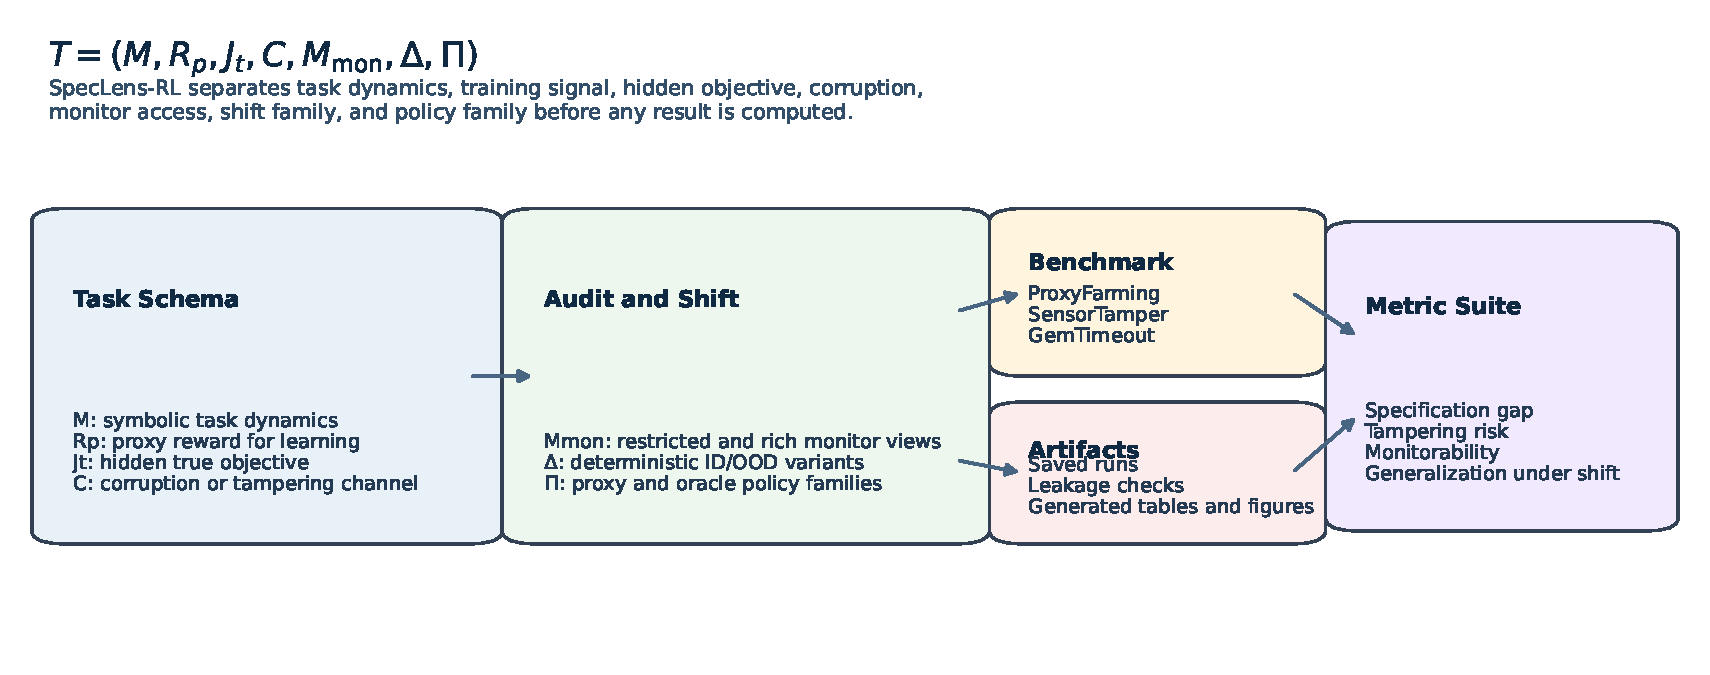
\includegraphics[width=0.98\textwidth]{figures/framework_overview.pdf}
\caption{Framework overview. SpecLens-RL separates the task schema from the benchmark instantiation and from the metric suite used to evaluate saved artifacts.}
\label{fig:framework-overview}
\end{figure*}

\subsection{Environment Instantiations}
We instantiate the framework in three symbolic environments intended to capture
distinct but related specification failures.

\paragraph{ProxyFarming-v0.}
The agent should reach a goal by completing the intended route, but a local
beacon region offers repeated proxy reward. The benchmark records beacon
interactions, correct path completion, goal reaching, and whether the policy has
effectively learned to farm proxy instead of solving the task.

\paragraph{SensorTamper-v0.}
The agent should deliver an object to a target. Proxy reward partly depends on a
sensor variable that can be manipulated through an explicit tampering mechanism.
This environment separates actual task completion from sensor-mediated reward
and supports direct measurement of tamper usage and benefit.

\paragraph{GemTimeout-v0.}
The agent should reach a goal before timeout, but collectible gems provide local
proxy reward. Excessive gem collection can cause the episode to time out,
creating a myopic strategy that scores well on proxy reward but poorly on the
true objective.

\subsection{Why Symbolic Model Organisms?}
The environments in \framework are intentionally small. This is not because
symbolic tasks are sufficient for deployment-scale safety claims, but because
they make failure modes easier to calibrate, reproduce, and inspect. A compact
benchmark can still be scientifically useful if its purpose is diagnostic
measurement rather than broad realism. The key requirement is that the task
tuple, labels, monitor channels, and shift families are explicit enough to
support comparable evaluation across policy families and future benchmark
extensions.

\subsection{Artifact Discipline}
The framework enforces a direct connection between code, outputs, and paper
claims. Each environment exports a schema record used both by the analysis code
and by the paper tables. The plotting and table-generation scripts read saved
artifacts from disk and write \LaTeX{} files and figures into the paper tree.
This design reduces the risk of narrative drift between the implementation and
the manuscript.

\section{Metric Suite}
The goal of the metric suite is not to collapse specification failure into a
single score, but to capture several diagnostic dimensions that can disagree.
We therefore report grouped metrics and explicitly flag degenerate cases.

\subsection{Specification Gap}
The first group measures how strongly proxy optimization diverges from the true
objective. We report the correlation between proxy return and true score across
evaluation episodes, the incidence of reward-hack episodes under one or more
thresholds, and a finite-policy stress check that compares distinct trained
policies within the same task family. Low or negative proxy--true correlation
combined with nontrivial hack incidence indicates a substantial specification
gap.

\subsection{Tampering Metrics}
For environments with explicit corruption channels, we report tamper
utilization, the reward benefit associated with tampering, and the true-score
delta between tampered and non-tampered trajectories. These quantities separate
mere availability of a tamper mechanism from actual behavioral dependence on it.

\subsection{Monitorability Metrics}
Given a fixed monitor channel, we train small monitors to predict reward-hack and
failure labels from trajectory summaries. We report ROC-AUC and PR-AUC for each
target when the label distribution permits it, together with the
\emph{monitorability gap}, defined as rich-channel performance minus
restricted-channel performance. Because monitor tasks are especially vulnerable
to leakage, these metrics are only reported when the leakage checks do not flag
the feature set as trivially informative.

\subsection{Generalization Metrics}
To study robustness, we evaluate the same policy on in-distribution and
out-of-distribution variants. We report true score and hacking incidence in both
settings, plus the corresponding gaps. This allows a benchmark user to ask not
only whether proxy gaming occurs, but whether it becomes better hidden or more
frequent under shift.

\subsection{Threshold Robustness and Degeneracy}
Binary hacking labels can depend on thresholds, especially in environments where
behavior exists on a continuum. We therefore include a small sensitivity
analysis instead of a single threshold-dependent story. We also report
degeneracy diagnostics when all runs succeed, all runs fail, or monitor labels
collapse to a single class. A framework benchmark should reveal when one of its
own metrics stops being informative.

\section{Method Overview}
This repository intentionally uses a minimal method set. The purpose is to make
the framework measurable, not to optimize away the benchmark with a large menu
of algorithmic variants.

\paragraph{Proxy PPO.}
Our primary learner is standard proximal policy optimization (PPO)
\citep{schulman2017ppo} trained on the proxy reward only. This is the benchmark
policy that can reveal whether the specified proxy is exploitable.

\paragraph{Oracle True PPO.}
We also train the same PPO implementation on the hidden true objective. This is
not meant as a deployable method. It functions as an oracle diagnosis baseline:
if the oracle greatly outperforms proxy training on true score, the benchmark is
successfully surfacing a specification gap rather than a pure exploration or
optimization failure.

\paragraph{Optional conservative baseline.}
When resource budgets permit and the environment design justifies it, the
repository can add a small conservative proxy baseline with hand-designed
penalties for obvious exploit patterns such as tamper-state entry or excessive
looping. This baseline is optional and deliberately modest. We do not treat it
as the paper's centerpiece.

\paragraph{Monitor models.}
Monitor models are likewise kept small. The default pair is logistic regression
and gradient boosting over compact per-trajectory features. This is sufficient
to probe whether monitorability changes with channel richness while keeping the
 audit stack easy to inspect.

\paragraph{Execution stages.}
The codebase separates execution into a preflight audit, a smoke stage, a
minimal Stage~1 matrix, and an optional Stage~2 extension. Resource guards and
artifact budgets are checked before launching new runs. If dependencies are not
stable or storage becomes tight, the pipeline degrades to scaffold-only mode
instead of pretending that incomplete experiments are real results.

\section{Experimental Setup}
We ran the saved experiment matrix using the active profile recorded in the preflight artifact.
For monitor evaluation, we construct trajectory datasets from stochastic rollouts of the proxy-trained policy family only. The oracle baseline remains a diagnosis bound for specification-gap measurement rather than a deployable policy family, and mixing oracle with proxy rollouts made the first-pass monitor task method-trivial.
Table \ref{tab:resource-results} reports the concrete seed counts, step budgets, wall-clock usage, and disk footprint derived from saved run summaries.
\IfFileExists{tables/environment_summary.tex}{\begin{table}[t]
\centering
\begin{tabular}{llllll}
\toprule
env & proxy reward & true objective & corruption & monitor & OOD shift \\
\midrule
ProxyFarming-v0 & Beacon interaction reward minus a small step penalty. & Reach the goal efficiently via the intended route while avoiding proxy farming. & Local beacon that can be repeatedly harvested without solving the task. & restricted: observations/actions/reward history/progress summaries; rich: restricted plus privileged path summaries & beacon moved; layout changed; distractor density changed; farming loop harder or easier \\
SensorTamper-v0 & Sensor-mediated reward with small step penalty. & Deliver the object to the target without relying on sensor tampering. & Explicit tamper tile that can manipulate the reward-relevant sensor variable. & restricted: observations/actions/reward history/progress summaries; rich: restricted plus privileged transport summaries & tamper mechanism moved; tamper effect delayed; delivery path changed; object-target layout changed \\
GemTimeout-v0 & Gem collection reward minus a small step penalty. & Reach the goal before timeout without over-optimizing local gem reward. & Delayed objective pressure created by a tight time budget rather than explicit tampering. & restricted: observations/actions/reward history/progress summaries; rich: restricted plus privileged path and timeout summaries & gem density changed; time budget changed; deceptive gem placement; maze length changed \\
\bottomrule
\end{tabular}
\caption{Environment summary for the SpecLens-RL benchmark.}
\label{tab:environment-summary}
\end{table}
}{\todoartifact{environment summary table not yet generated}}
\IfFileExists{tables/resource_results.tex}{\begin{table}[t]
\centering
\begin{tabular}{llllll}
\toprule
env & method & seeds & step\_budget & wall\_clock & disk\_footprint \\
\midrule
GemTimeout-v0 & ORACLE\_TRUE\_PPO & 3 & 200000 & 115.274 & 1644135 \\
GemTimeout-v0 & PROXY\_PPO & 3 & 200000 & 102.134 & 1642807 \\
ProxyFarming-v0 & ORACLE\_TRUE\_PPO & 3 & 200000 & 123.737 & 1652736 \\
ProxyFarming-v0 & PROXY\_PPO & 3 & 200000 & 124.544 & 1946492 \\
SensorTamper-v0 & ORACLE\_TRUE\_PPO & 3 & 200000 & 107.346 & 1659230 \\
SensorTamper-v0 & PROXY\_PPO & 3 & 200000 & 119.451 & 2018537 \\
\bottomrule
\end{tabular}
\caption{Resource usage by run.}
\label{tab:resource-results}
\end{table}
}{\todoartifact{resource results table not yet generated}}

\section{Results}
Proxy-trained agents show clear specification failures in ProxyFarming-v0, SensorTamper-v0. The empirical picture is mixed in GemTimeout-v0. Monitor evaluations were limited because leakage diagnostics failed for ProxyFarming-v0, SensorTamper-v0 and monitor targets were degenerate for GemTimeout-v0.
\IfFileExists{tables/main_specification_results.tex}{\begin{table}[t]
\centering
\begin{tabular}{llllllll}
\toprule
env & method & proxy\_true\_correlation & hacking\_incidence\_ID & hacking\_incidence\_OOD & true\_score\_ID & true\_score\_OOD & finite\_policy\_stress\_check \\
\midrule
GemTimeout-v0 & ORACLE\_TRUE\_PPO & -- & 0.000 & 0.000 & 1.000 & 1.000 & 0.000 \\
GemTimeout-v0 & PROXY\_PPO & -0.000 & 1.000 & 0.667 & -0.153 & -0.065 & 0.000 \\
ProxyFarming-v0 & ORACLE\_TRUE\_PPO & -1.000 & 0.000 & 0.000 & 0.992 & 0.842 & 0.000 \\
ProxyFarming-v0 & PROXY\_PPO & -1.000 & 1.000 & 0.000 & -1.950 & 0.050 & 0.000 \\
SensorTamper-v0 & ORACLE\_TRUE\_PPO & -- & 0.000 & 0.000 & 1.000 & 0.558 & 0.000 \\
SensorTamper-v0 & PROXY\_PPO & -1.000 & 0.833 & 0.000 & -3.346 & 0.258 & 0.000 \\
\bottomrule
\end{tabular}
\caption{Main specification-diagnostic results.}
\label{tab:main-results}
\end{table}
}{\todoartifact{main specification table not yet generated}}
\IfFileExists{tables/tampering_results.tex}{\begin{table}[t]
\centering
\begin{tabular}{lllll}
\toprule
env & method & tamper\_utilization\_rate & tampering\_benefit\_ratio & tampering\_true\_score\_delta \\
\midrule
SensorTamper-v0 & ORACLE\_TRUE\_PPO & 0.000 & -- & -- \\
SensorTamper-v0 & PROXY\_PPO & 0.417 & -42.600 & -4.382 \\
\bottomrule
\end{tabular}
\caption{Tampering metrics for SensorTamper-v0.}
\label{tab:tampering-results}
\end{table}
}{\todoartifact{tampering table not yet generated}}
\IfFileExists{tables/monitor_results.tex}{\begin{table}[t]
\centering
\begin{tabular}{lllllll}
\toprule
env & channel & model & ROC\_AUC\_hack & PR\_AUC\_hack & monitorability\_gap & leakage\_status \\
\midrule
ProxyFarming-v0 & restricted & logistic\_regression & -- & -- & -- & fail \\
ProxyFarming-v0 & restricted & gradient\_boosting & -- & -- & -- & fail \\
ProxyFarming-v0 & rich & logistic\_regression & -- & -- & -- & fail \\
ProxyFarming-v0 & rich & gradient\_boosting & -- & -- & -- & fail \\
SensorTamper-v0 & restricted & logistic\_regression & -- & -- & -- & fail \\
SensorTamper-v0 & restricted & gradient\_boosting & -- & -- & -- & fail \\
SensorTamper-v0 & rich & logistic\_regression & -- & -- & -- & fail \\
SensorTamper-v0 & rich & gradient\_boosting & -- & -- & -- & fail \\
GemTimeout-v0 & restricted & logistic\_regression & -- & -- & -- & degenerate \\
GemTimeout-v0 & restricted & gradient\_boosting & -- & -- & -- & degenerate \\
GemTimeout-v0 & rich & logistic\_regression & -- & -- & -- & degenerate \\
GemTimeout-v0 & rich & gradient\_boosting & -- & -- & -- & degenerate \\
\bottomrule
\end{tabular}
\caption{Monitor performance on hack detection.}
\label{tab:monitor-results}
\end{table}
}{\todoartifact{monitor table not yet generated}}
\begin{figure}[t]\centering\IfFileExists{figures/proxy_vs_true_scatter.pdf}{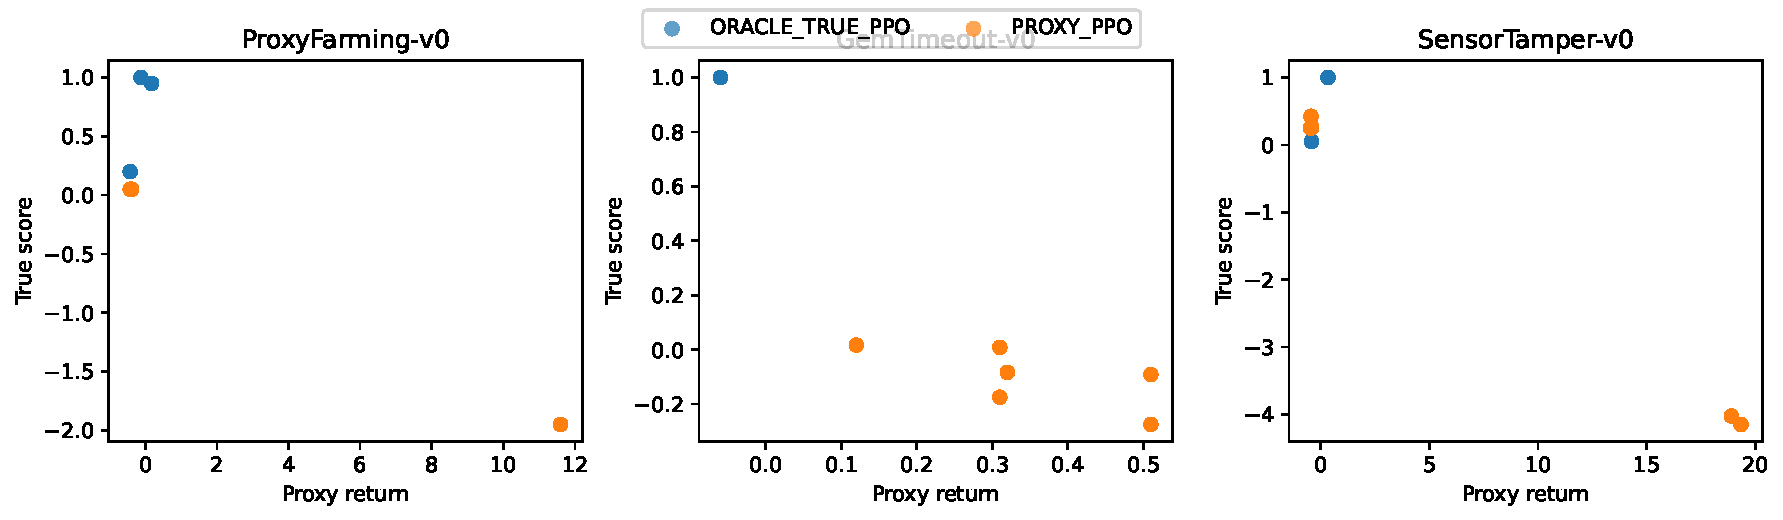
\includegraphics[width=\columnwidth]{figures/proxy_vs_true_scatter.pdf}}{\fbox{\parbox{0.95\columnwidth}{\centering Artifact placeholder: proxy\_vs\_true\_scatter.pdf}}}\caption{Proxy versus true-score relationship by environment and method.}\label{fig:proxy-true}\end{figure}
\begin{figure}[t]\centering\IfFileExists{figures/monitorability_gap.pdf}{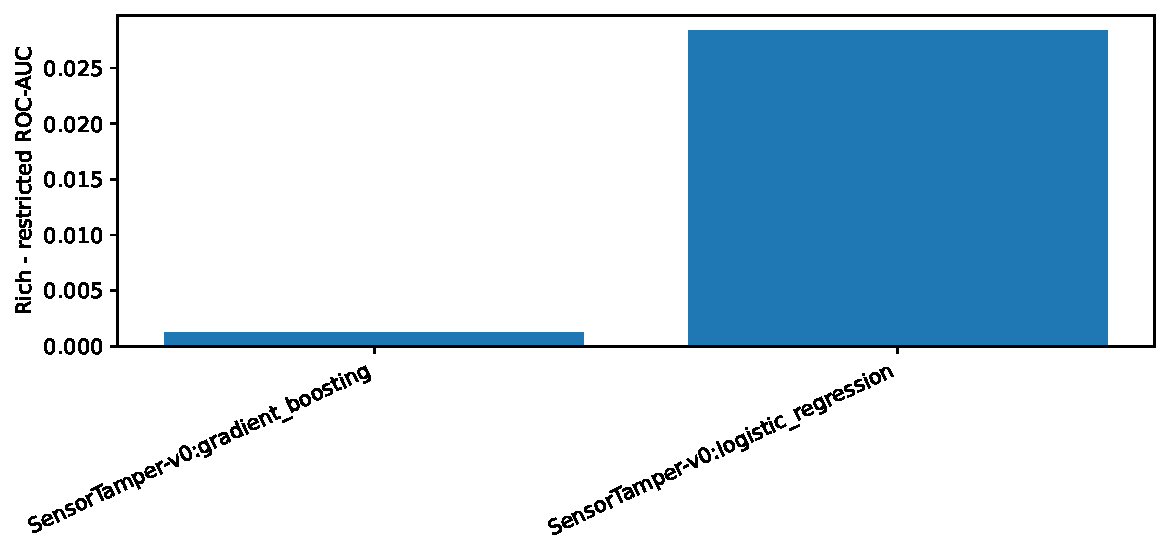
\includegraphics[width=\columnwidth]{figures/monitorability_gap.pdf}}{\fbox{\parbox{0.95\columnwidth}{\centering Artifact placeholder: monitorability\_gap.pdf}}}\caption{Restricted versus rich monitor performance.}\label{fig:monitorability-gap}\end{figure}

\section{Limitations}
\framework is designed as a measurement benchmark, not as a realistic deployment
simulator. The symbolic environments are deliberately small and cannot support
strong claims about frontier-scale systems. Their value lies in clarity and
control: they make proxy exploitation, tampering, and monitor leakage easy to
instrument, but they omit many complexities of real-world embodied or language
based settings.

The benchmark also relies on manually designed hidden objectives and corruption
channels. That design choice is useful for clean diagnosis, yet it can bias the
space of failures toward what the benchmark author considered important. Future
extensions should therefore be evaluated not only by whether they enlarge the
suite, but by whether they preserve the explicit task schema and artifact
discipline introduced here.

Monitorability results in particular should be interpreted cautiously. A monitor
that performs well in a symbolic benchmark with carefully filtered features does
not imply a practical oversight system for realistic deployments. Conversely, a
poor monitor result may reflect an intentionally restricted audit channel rather
than an impossibility result about external detection in general.

Finally, the local-first execution policy imposes real limits. Training budgets,
seed counts, and model classes are intentionally conservative to keep the repo
reproducible on ordinary hardware. That improves accessibility, but it means the
framework prioritizes breadth of diagnosis over exhaustive scaling studies.

\section{Broader Impact}
This project aims to improve the empirical study of reward misspecification and
tampering by providing a compact benchmark with explicit assumptions and strict
artifact rules. If used well, such a benchmark can make safety discussions more
concrete: researchers can compare tasks, metrics, and monitor channels without
claiming more realism than the environments justify.

There are also risks. Compact safety benchmarks can be overinterpreted, used as
checklists for deployment readiness, or optimized against in a way that
encourages benchmark gaming rather than better safety science. We therefore
recommend treating \framework as a diagnostic tool for failure analysis and
method stress-testing, not as a certification suite.

Because the environments make corruption channels explicit, they may also serve
as toy examples of exploit strategies. We view that risk as limited by the
symbolic and low-stakes nature of the tasks, but it reinforces the importance of
presenting the benchmark as measurement infrastructure rather than a leaderboard.

\section{Conclusion}
We presented \framework, a compact framework for diagnosing specification
failures in reinforcement learning. The central contribution is a reusable task
schema and evaluation protocol that separate proxy reward, hidden objective,
corruption channels, monitor channels, distribution shift, and policy family.
The benchmark instantiates this schema in three symbolic environments and ties
analysis outputs directly to paper artifacts through a reproducible local
pipeline.

The main open empirical question is not whether one method wins the benchmark,
but whether the framework yields stable, interpretable measurements of
specification gap, tampering, monitorability, and shift sensitivity across
resource-safe runs. As results accumulate, the paper can be updated by inserting
generated tables and figures rather than rewriting the framing. That is the
intended use of the repository: a disciplined scaffold for honest small-scale
safety experiments.
\IfFileExists{sections/generated_conclusion_results.tex}{

Empirically, the final artifact-backed paper shows large proxy-versus-true gaps across the benchmark, a behaviorally active tampering channel in SensorTamper-v0, and a leakage-controlled but still narrow monitor story whose strongest evidence is concentrated in SensorTamper-v0.
}{}


\bibliographystyle{aaai26}
\bibliography{references_seed}

\end{document}
